\section{Data Transfer Methods}
\label{sec:data_transfer_methods}

In this section, we investigate data transfer methods for the GPU.
A standard data transfer method uses hardware DMA engines integrated on
the GPU, while direct data read and write accesses to the GPU device
memory are allowed through PCIe BARs.
We can also use microcontrollers integrated on the GPU to send and
receive data across the host and the device memory.
Unfortunately, only a limited piece of these schemes has been studied in
the literature.
Our investigation and open implementations of these schemes provide a
better understanding of data transfer mechanisms for the GPU.
Note that we restrict our attention to the NVIDIA GPU architecture, but
the concepts of data transfer methods introduced in this paper are
mostly applicable to PCIe-connected compute devices.

\subsection{Standard DMA}
\label{sec:dma}

\begin{figure}[!t]
 \centering
 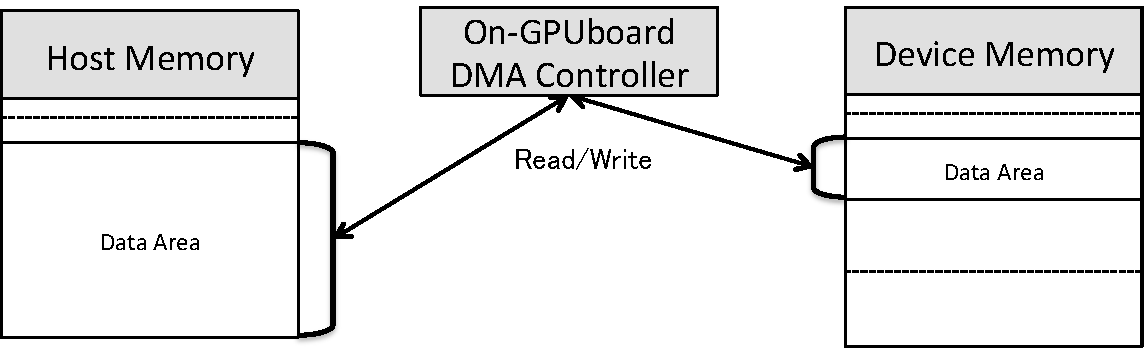
\includegraphics[width=0.4\textwidth]{figure/Method/DMA_Method.pdf}
 \caption{Standard DMA.}
 \label{fig:dma}
\end{figure}

The most typical method for GPU data transfers is to use standard DMA
engines integrated on the GPU.
There are two types of such DMA engines for synchronous and asynchronous
data transfer operations respectively.
We focus on the synchronous DMA engines, which always operate in a
sequential fashion with compute engines.

Figure~\ref{fig:dma} shows a concept of this standard DMA method.
To perform this DMA, we write \textit{GPU commands} to an on-board DMA
engine.
Upon a request of GPU commands, the DMA engine transfers a specified
data set between the host and the device memory.
Once a DMA transfer starts, it is non-preemptive.
This method is often the most effective to transfer a large size of
data.
Details of the GPU DMA mechanism can be found in previous
work~\cite{Kato_ATC11, Kato_ATC12}.

\subsection{Microcontroller-based Data Transfer}
\label{sec:micro}

\begin{figure}[!t]
 \centering
 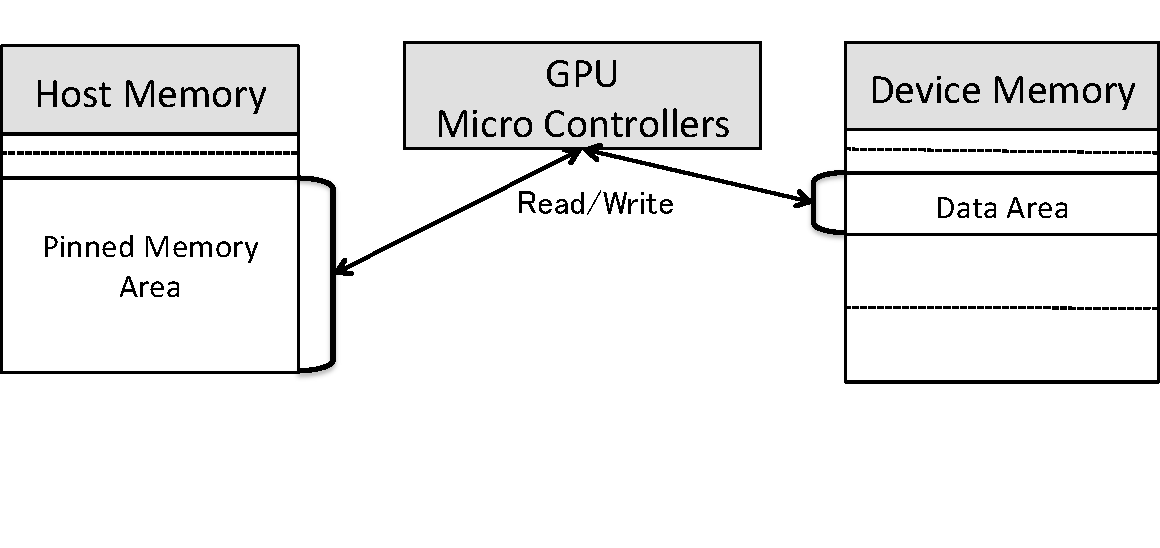
\includegraphics[width=0.4\textwidth]{figure/Method/Micro_Method.pdf}
 \caption{Microcontroller-based data transfer.}
 \label{fig:micro}
\end{figure}

The GPU provides on-board microcontrollers to control GPU functional
units (compute, DMA, power, temperature, encode, decode, etc.).
Albeit tiny hardware, these microcontrollers are available for GPU
resource management beyond just controlling the functional units.
Each microcontroller supports special instructions to transfer data in
the data sections to and from the host or the device memory.
The data transfer is offloaded to the microcontroller, \textit{i.e.},
DMA, but is controlled by the microcontroller itself.
Leveraging this mechanism, we can provide data communications between
the host and the device memory.

Figure~\ref{fig:micro} shows a concept of this microcontroller-based
data transfer method.
Since there is no data path to directly copy data between the host and
the device memory using a microcontroller, each data transfer needs
to take two hops: (i) the host memory and a microcontroller and (ii) the
device memory and a microcontroller.
This is non-trivial overhead but the handling of this DMA is very
light-weight as compared to the standard DMA method.

The microcontroller is executing firmware loaded by the device driver.
We modify this firmware code to employ an interface for the data
communications.
The firmware adopts an event-driven design: it invokes only when the
device driver sends some command from the CPU.
The user program hence first needs to communicate with the device driver
to issue such a command.
Our implementation uses \texttt{ioctl} system calls to achieve this user
and device driver communication.

\subsection{Memory-mapped Read and Write}
\label{sec:iorw}

\begin{figure}[!t]
 \centering
 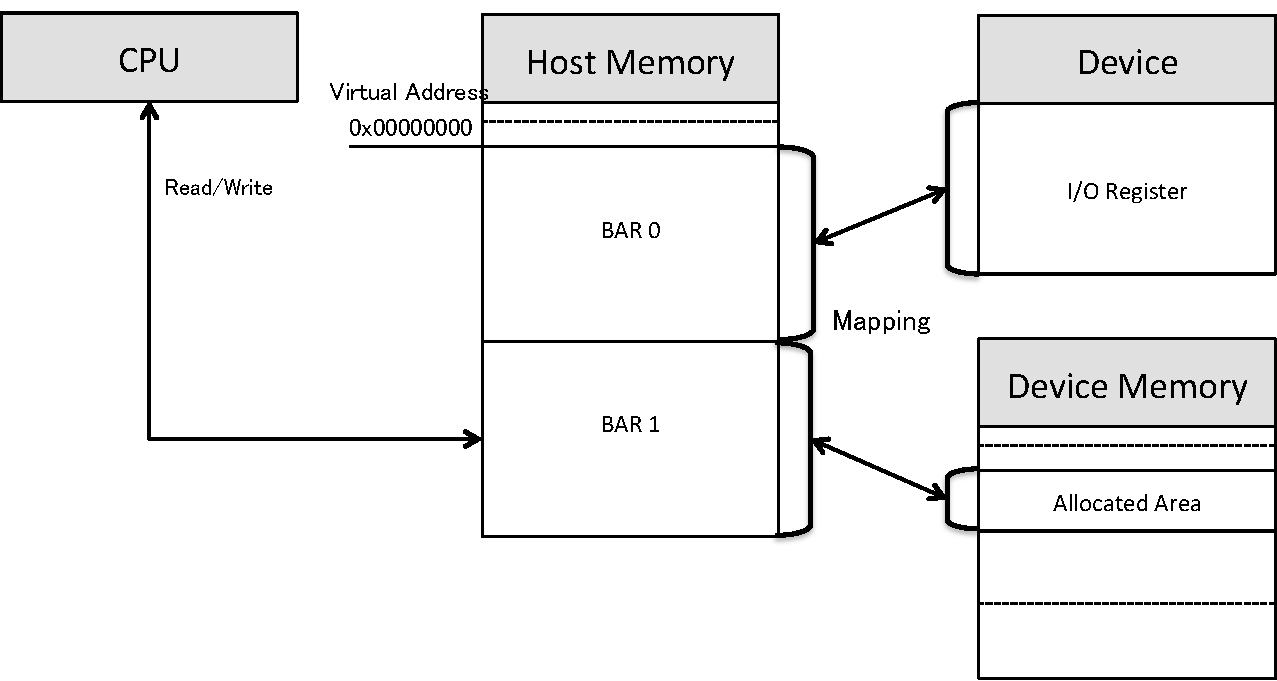
\includegraphics[width=0.4\textwidth]{figure/Method/IORW_Method.pdf}
 \caption{Memory-mapped read and write.}
 \label{fig:iorw}
\end{figure}

The aforementioned two methods are based on DMA functions.
DMA is usually high-throughput but it inevitably incurs overhead in the
setup.
A small size of data transfers may encounter severe latency problems due
to this overhead.
One of good examples can be found in the plasma control
system~\cite{Kato_ICCPS13}.
If low-latency is required, direct read and write accesses are more
appropriate than hardware-based DMA.
Since the GPU as a PCIe-connected device provides memory-mapped regions
upon the PCI address space, the CPU can directly access the device
memory without using bounce buffers on the host memory.

Figure~\ref{fig:iorw} shows a concept of this memory-mapped read and
write method.
NVIDIA GPUs as well as most other PCIe devices expose base address
registers (BARs) to the system, through which the CPU can access
specific areas of the device memory.
There are several BARs depending on the target device.
NVIDIA GPUs typically provide the following BARs:
\begin{description}
 \item[BAR0] Memory-mapped I/O (MMIO) registers.
 \item[BAR1] Device memory aperture (windows).
 \item[BAR2] I/O port or complementary space of BAR1.
 \item[BAR3] Same as BAR2.
 \item[BAR5] I/O port.
 \item[BAR6] PCI ROM.
\end{description}

Often the BAR0 is used to access the control registers of the GPU while
the BAR1 makes the device memory visible to the CPU.
This direct read and write method is pretty simple.
We create virtual address space for the BAR1 region and set its leading
address to a specific control register.
Thus the BAR1 region can be directly accessed by the GPU using the
unified memory addressing (UMA) mode, where all memory objects allocated
to the host and the device memory can be referenced by the same address
space.
Once the BAR1 region is mapped, all we have to do is to manage the page
table of the GPU to allocate memory objects from this BAR1 region and
call the I/O remapping function supported by the OS kernel to remap the
corresponding BAR1 region to the user-space buffer.

\subsection{Memory-window Read and Write}
\label{sec:memwnd}

\begin{figure}[!t]
 \centering
 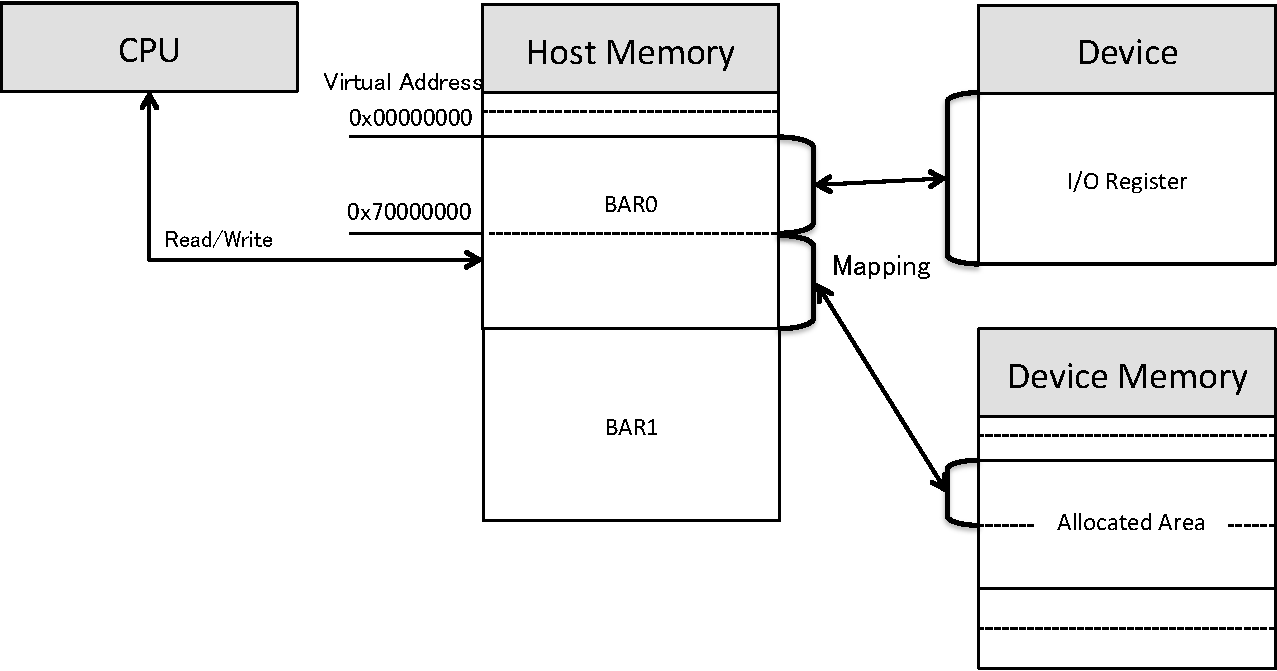
\includegraphics[width=0.4\textwidth]{figure/Method/MEMWND_Method.pdf}
 \caption{Memory-window read and write.}
 \label{fig:memwnd}
\end{figure}

The BAR0 region is often called memory-mapped I/O (MMIO) space.
This is the main control space of the GPU, through which all hardware
engines are controlled.
Its space is sparsely populated with areas representing individual
hardware engines, which in turn are sparsely populated with control
registers.
The list of hardware engines is architecture-dependent.
The MMIO space contains a special subarea for indirect device and host
memory accesses, seperated from the control registers.
This plays a role of windows that make the device memory visible to the
CPU in a different way than the BAR1 region.

Figure~\ref{fig:memwnd} shows a concept of this memory-window read and
write method.
To set the memory window, we obtain the leading physical address of the
corresponding memory object and set it to a specific control register.
By doing so, a limited range of the memory object becomes visible to the
CPU through a specific BAR0 region.
In case of NVIDIA GPUs, the size of this range is $4$MB and the specific
BAR0 region begins at 0x70000000 in the MMIO address.
Once the window is set, we can read and write this BAR0 region to access
data on the device memory.

\subsection{Pinned Host Memory}

Yet another approach to GPU data transfers is to use the pinned host
memory.
As aforementioned, NVIDIA GPUs support UMA.
This is due to the graphics address remapping table (GART) employed by
the GPU, allowing the system to specify physical host memory addresses
directly in the GPU page table as far as they are associated with pinned
PCI-mapped pages.
Although this approach is also effective to an extent for low-latency
GPU computing~\cite{Kato_ICCPS13}, it is not within the scope of this
paper and we focus on how to access the device memory in this paper.
